\documentclass[11pt]{article}

\usepackage[margin=1in]{geometry}
\usepackage{setspace}
\usepackage{amsmath,amssymb,amsthm,mathtools}
\usepackage{bm}
\usepackage{graphicx}
\usepackage{float}
\usepackage{enumitem}
\usepackage{booktabs}
\usepackage{hyperref}
\usepackage[nameinlink,capitalize]{cleveref}
\usepackage{natbib}

\onehalfspacing

\title{A Simple Dynamic Model of Industrial Policy \\ for Supply-Chain Resilience}
\author{Hung D. Hoang}
\date{January 2026}

\begin{document}

\maketitle

\begin{center}
\textbf{Project Repository:} \url{https://github.com/dhhoang-vna/Dynamic-Programming-Project}
\end{center}

\section{Motivation}

Recent work in international economics has emphasized that the key policy problem in a fragmented world is not only static protection, but also the dynamic trade-off between efficiency and resilience. Foreign sourcing may be cheaper in normal times, yet domestic capacity can be valuable as insurance when foreign supply is disrupted. This tension appears in recent research on diversification versus reshoring, forward-looking resilience investment in supply chains, and the possibility that decentralized economies underinvest in resilience relative to the social optimum \citep{GHL2023,GHS2024,CDS2024}.

Motivated by this literature, I study a simple dynamic planner problem in which the government chooses an industrial policy instrument that raises domestic productive capacity in a strategic upstream sector. The benefit of policy is that greater domestic capacity reduces future exposure to costly foreign disruptions; the cost is that industrial policy is fiscally costly and domestic production may be intrinsically more expensive than foreign sourcing in normal times.

The purpose of the model is not to reproduce the full richness of recent supply-chain models, but to provide a tractable dynamic programming framework with clear state variables, control variables, a Bellman equation, and first-order conditions.

\section{Environment}

Time is discrete, indexed by $t=0,1,2,\dots$. There is a benevolent social planner and a representative domestic strategic-input sector. The economy requires one unit of a critical intermediate input each period in order to produce final output.

\subsection{Supply of the strategic input}

The required unit of input can be obtained from two sources:
\begin{itemize}[leftmargin=2em]
    \item domestic production, denoted $x_t$,
    \item foreign sourcing, denoted $1-x_t$.
\end{itemize}
Hence feasibility requires
\begin{equation}
0 \le x_t \le 1.
\end{equation}

Domestic production is constrained by installed domestic capacity $K_t$, so
\begin{equation}
x_t \le K_t.
\end{equation}
I restrict attention to $K_t \in [0,1]$, since total required input is normalized to one.

\subsection{Domestic production cost}

Domestic production is costly. For tractability, I assume a convex cost function:
\begin{equation}
C^d(x_t) = \frac{c_d}{2}x_t^2, \qquad c_d >0.
\end{equation}
This captures increasing marginal cost of domestic sourcing.

\subsection{Foreign sourcing cost and disruption risk}

Foreign sourcing is cheaper in normal times but vulnerable to disruption. Let $d_t \in \{0,1\}$ denote the disruption state:
\[
d_t =
\begin{cases}
0 & \text{no disruption},\\
1 & \text{disruption}.
\end{cases}
\]
The foreign per-unit sourcing cost is
\begin{equation}
p_f(d_t)=
\begin{cases}
p_L & \text{if } d_t=0,\\
p_H & \text{if } d_t=1,
\end{cases}
\qquad p_H>p_L>0.
\end{equation}
Thus the foreign sourcing cost is
\begin{equation}
C^f(x_t,d_t)=p_f(d_t)(1-x_t).
\end{equation}

The disruption state follows a Markov process:
\begin{equation}
\Pr(d_{t+1}=1 \mid d_t=0)=\pi_{01}, \qquad
\Pr(d_{t+1}=0 \mid d_t=1)=\pi_{10},
\end{equation}
with $\pi_{01},\pi_{10}\in(0,1)$.

\subsection{Industrial policy and capacity accumulation}

The planner chooses an industrial policy instrument $s_t \ge 0$, interpreted as a subsidy or public support effort that raises domestic productive capacity. Capacity evolves according to
\begin{equation}
K_{t+1}=(1-\delta)K_t+\psi s_t,
\qquad \delta \in (0,1), \ \psi>0.
\end{equation}
Here $\delta$ is depreciation or obsolescence, and $\psi$ measures the effectiveness of policy.

The fiscal cost of industrial policy is assumed convex:
\begin{equation}
\Phi(s_t)=\frac{\gamma}{2}s_t^2,
\qquad \gamma>0.
\end{equation}

\subsection{Flow welfare}

Let $A>0$ denote the gross benefit from final production, which is constant because the economy always obtains the required unit of the strategic input. Then period welfare is
\begin{equation}
u(K_t,d_t;x_t,s_t)
=
A-\frac{c_d}{2}x_t^2-p_f(d_t)(1-x_t)-\frac{\gamma}{2}s_t^2.
\end{equation}
The first term is the gross benefit of production; the remaining terms are domestic production cost, foreign sourcing cost, and fiscal cost of policy.

\section{Planner Problem}

The planner chooses sequences $\{x_t,s_t\}_{t\ge 0}$ to maximize expected discounted welfare:
\begin{equation}
\max_{\{x_t,s_t\}_{t\ge 0}}
\mathbb{E}_0
\sum_{t=0}^{\infty}
\beta^t
\left[
A-\frac{c_d}{2}x_t^2-p_f(d_t)(1-x_t)-\frac{\gamma}{2}s_t^2
\right],
\end{equation}
subject to
\begin{align}
0 \le x_t \le K_t, \\
s_t \ge 0, \\
K_{t+1}=(1-\delta)K_t+\psi s_t,
\end{align}
and the Markov transition rule for $d_t$.

The planner internalizes the intertemporal value of domestic capacity. In normal times, foreign sourcing may be efficient because $p_L$ is relatively low. However, when a disruption occurs and the economy faces $p_H$, previously accumulated domestic capacity allows substitution away from foreign inputs. Thus industrial policy acts as a dynamic insurance device.

\section{Bellman Equation}

Let $V(K,d)$ denote the value function when the current state is $(K,d)$. The Bellman equation is
\begin{equation}
V(K,d)
=
\max_{x,s}
\left\{
A-\frac{c_d}{2}x^2-p_f(d)(1-x)-\frac{\gamma}{2}s^2
+\beta \mathbb{E}\left[V(K',d')\mid d\right]
\right\},
\end{equation}
subject to
\begin{align}
0 \le x \le K, \\
s \ge 0, \\
K'=(1-\delta)K+\psi s.
\end{align}

Since $d$ is Markov, the expectation can be written explicitly as
\begin{equation}
\mathbb{E}\left[V(K',d')\mid d\right]
=
\sum_{d'\in\{0,1\}}
\Pr(d' \mid d)\,V(K',d').
\end{equation}
Hence
\begin{equation}
V(K,d)
=
\max_{0\le x\le K,\ s\ge 0}
\left\{
A-\frac{c_d}{2}x^2-p_f(d)(1-x)-\frac{\gamma}{2}s^2
+\beta
\sum_{d'\in\{0,1\}}
\Pr(d'\mid d)\,
V\!\left((1-\delta)K+\psi s,d'\right)
\right\}.
\end{equation}

This recursive formulation makes the intertemporal trade-off transparent. A higher subsidy $s$ reduces current welfare through the fiscal cost $\frac{\gamma}{2}s^2$, but raises future domestic capacity and therefore future resilience.

\section{State and Control Variables}

The model has two state variables:
\begin{equation}
(K_t,d_t).
\end{equation}
They are:
\begin{itemize}[leftmargin=2em]
    \item $K_t$: installed domestic capacity in the strategic sector,
    \item $d_t$: the foreign disruption state.
\end{itemize}

The model has two control variables:
\begin{equation}
(x_t,s_t).
\end{equation}
They are:
\begin{itemize}[leftmargin=2em]
    \item $x_t$: domestic production of the critical input,
    \item $s_t$: industrial policy effort that builds future domestic capacity.
\end{itemize}

The law of motion for the endogenous state variable is
\begin{equation}
K_{t+1}=(1-\delta)K_t+\psi s_t.
\end{equation}

\section{FOCs and Interpretation}

The planner solves for $x_t$ and $s_t$ given the current state $(K_t,d_t)$. Because $x_t$ affects only the current payoff while $s_t$ affects future capacity, the problem is especially tractable.

\subsection{Optimal domestic sourcing decision}

Fix a state $(K,d)$. The planner chooses $x$ to solve
\begin{equation}
\max_{0\le x\le K}
\left[
-\frac{c_d}{2}x^2-p_f(d)(1-x)
\right].
\end{equation}
Equivalently, ignoring constants,
\begin{equation}
\max_{0\le x\le K}
\left[
p_f(d)x-\frac{c_d}{2}x^2
\right].
\end{equation}

If the capacity constraint does not bind, the first-order condition is
\begin{equation}
p_f(d)-c_d x = 0.
\end{equation}
Hence the unconstrained optimum is
\begin{equation}
x^{u}(d)=\frac{p_f(d)}{c_d}.
\end{equation}

Imposing the capacity constraint yields the policy rule
\begin{equation}
x^*(K,d)=\min\left\{K,\frac{p_f(d)}{c_d}\right\}.
\end{equation}

\paragraph{Interpretation.}
Domestic sourcing rises when foreign sourcing becomes more expensive. In particular, if a disruption raises foreign input costs from $p_L$ to $p_H$, the planner wants to substitute toward domestic production. However, this substitution is limited by installed domestic capacity $K$. This creates an intertemporal motive for industrial policy: capacity built in advance is valuable when disruptions arrive.

\subsection{Optimal industrial policy}

Now consider the subsidy choice. The Bellman equation implies the first-order condition
\begin{equation}
-\gamma s
+
\beta \psi
\sum_{d'\in\{0,1\}}
\Pr(d'\mid d)\,
V_K(K',d')
=0,
\end{equation}
where
\begin{equation}
K'=(1-\delta)K+\psi s.
\end{equation}

Thus, for an interior optimum,
\begin{equation}
\gamma s
=
\beta \psi
\sum_{d'\in\{0,1\}}
\Pr(d'\mid d)\,
V_K(K',d').
\end{equation}

\paragraph{Interpretation.}
The left-hand side is the marginal fiscal cost of industrial policy. The right-hand side is the discounted marginal continuation value of raising next period's domestic capacity. Therefore, the planner increases industrial policy until the current marginal fiscal cost equals the expected discounted marginal value of resilience.

\subsection{Envelope condition}

The value of domestic capacity is characterized by the envelope condition
\begin{equation}
V_K(K,d)
=
\frac{\partial u}{\partial K}
+
\beta(1-\delta)
\sum_{d'\in\{0,1\}}
\Pr(d'\mid d)\,
V_K(K',d').
\end{equation}

The direct term $\frac{\partial u}{\partial K}$ depends on whether the domestic capacity constraint binds.

\paragraph{Case 1: slack capacity.}
If
\begin{equation}
K > \frac{p_f(d)}{c_d},
\end{equation}
then the constraint does not bind and
\begin{equation}
x^*(K,d)=\frac{p_f(d)}{c_d}.
\end{equation}
In this case, a marginal increase in $K$ has no current-period payoff effect, so
\begin{equation}
\frac{\partial u}{\partial K}=0
\end{equation}
and therefore
\begin{equation}
V_K(K,d)
=
\beta(1-\delta)
\sum_{d'\in\{0,1\}}
\Pr(d'\mid d)\,
V_K(K',d').
\end{equation}

\paragraph{Case 2: binding capacity.}
If
\begin{equation}
K < \frac{p_f(d)}{c_d},
\end{equation}
then $x^*(K,d)=K$. Substituting into current utility,
\begin{equation}
u(K,d;s)
=
A-\frac{c_d}{2}K^2-p_f(d)(1-K)-\frac{\gamma}{2}s^2.
\end{equation}
Differentiating with respect to $K$,
\begin{equation}
\frac{\partial u}{\partial K}=p_f(d)-c_dK.
\end{equation}
Hence
\begin{equation}
V_K(K,d)
=
p_f(d)-c_dK
+
\beta(1-\delta)
\sum_{d'\in\{0,1\}}
\Pr(d'\mid d)\,
V_K(K',d').
\end{equation}

\paragraph{Interpretation.}
Domestic capacity is especially valuable when foreign disruptions make imports expensive and when the domestic capacity constraint binds. But the marginal value of capacity declines as $K$ rises, because the economy becomes less constrained.

\section{Numerical Results (VFI and PFI)}

This section reports the numerical policy and value functions computed in Python for the model above. I solve the Bellman problem using both value function iteration (VFI) and policy function iteration (PFI), and then plot the resulting objects as functions of domestic capacity $K$ under disruption states $d\in\{0,1\}$.

\subsection{Value Function}

\begin{figure}[H]
    \centering
    \begin{minipage}[t]{0.49\textwidth}
        \centering
        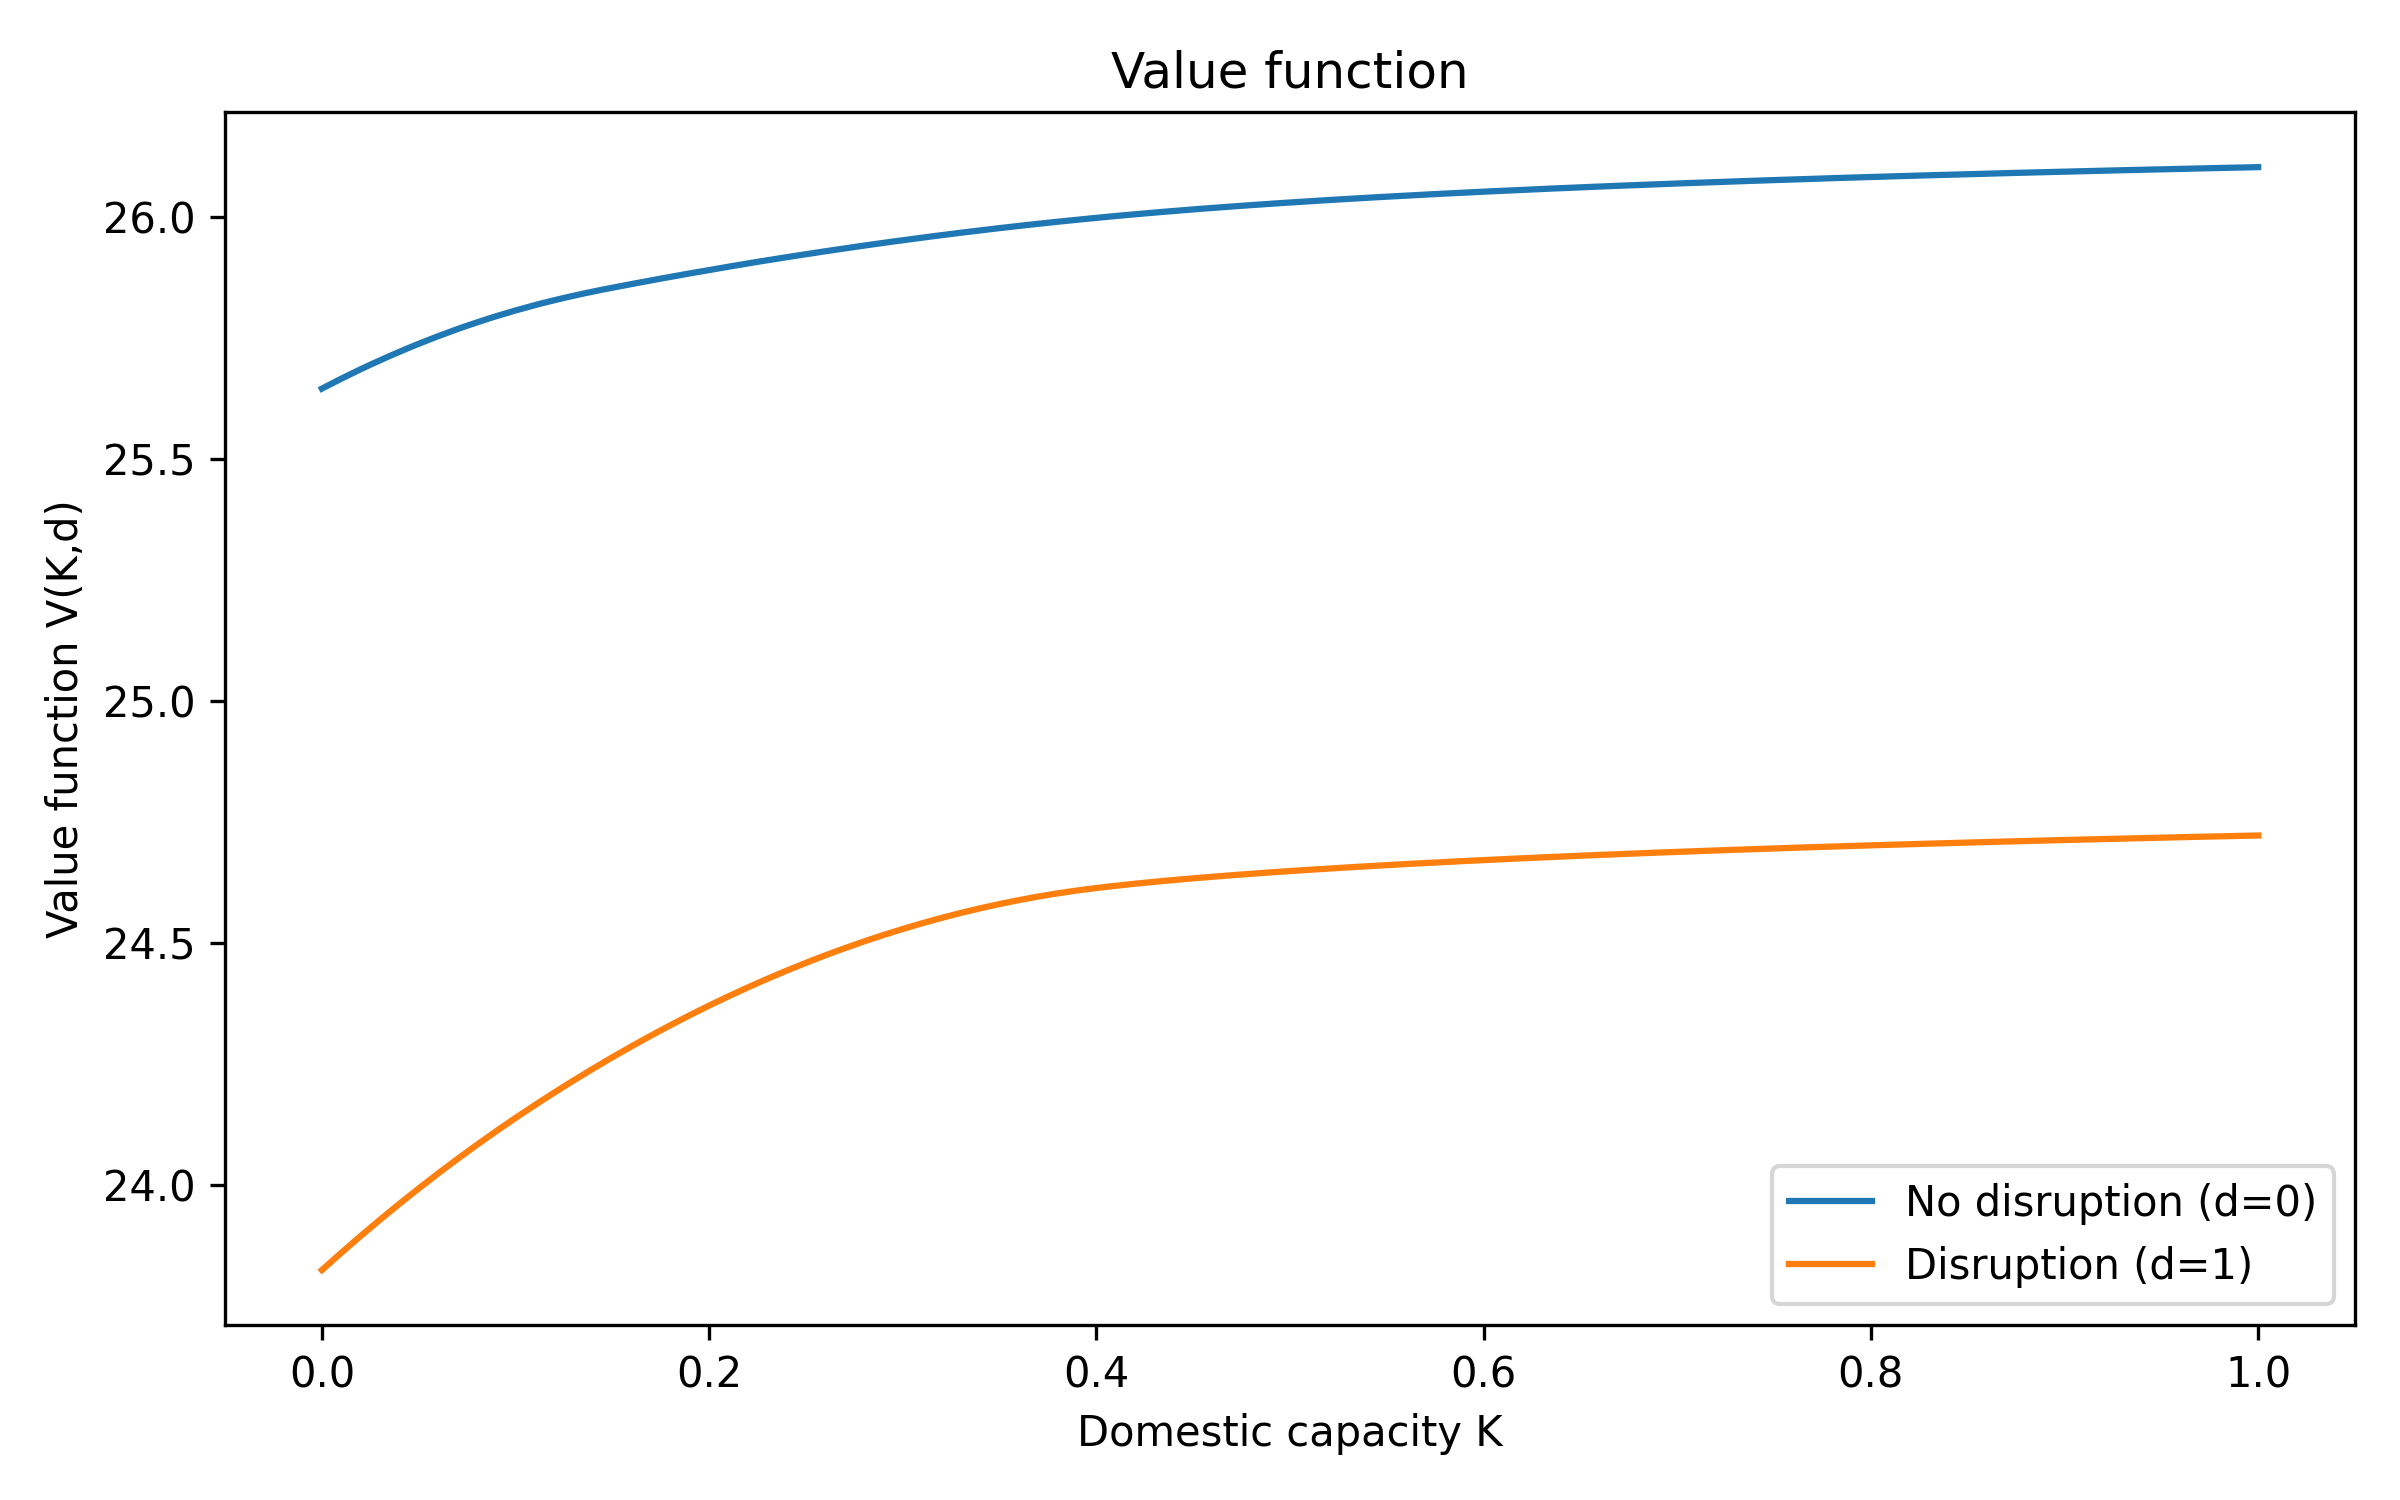
\includegraphics[width=\textwidth]{value_function.png}
    \end{minipage}
    \hfill
    \begin{minipage}[t]{0.49\textwidth}
        \centering
        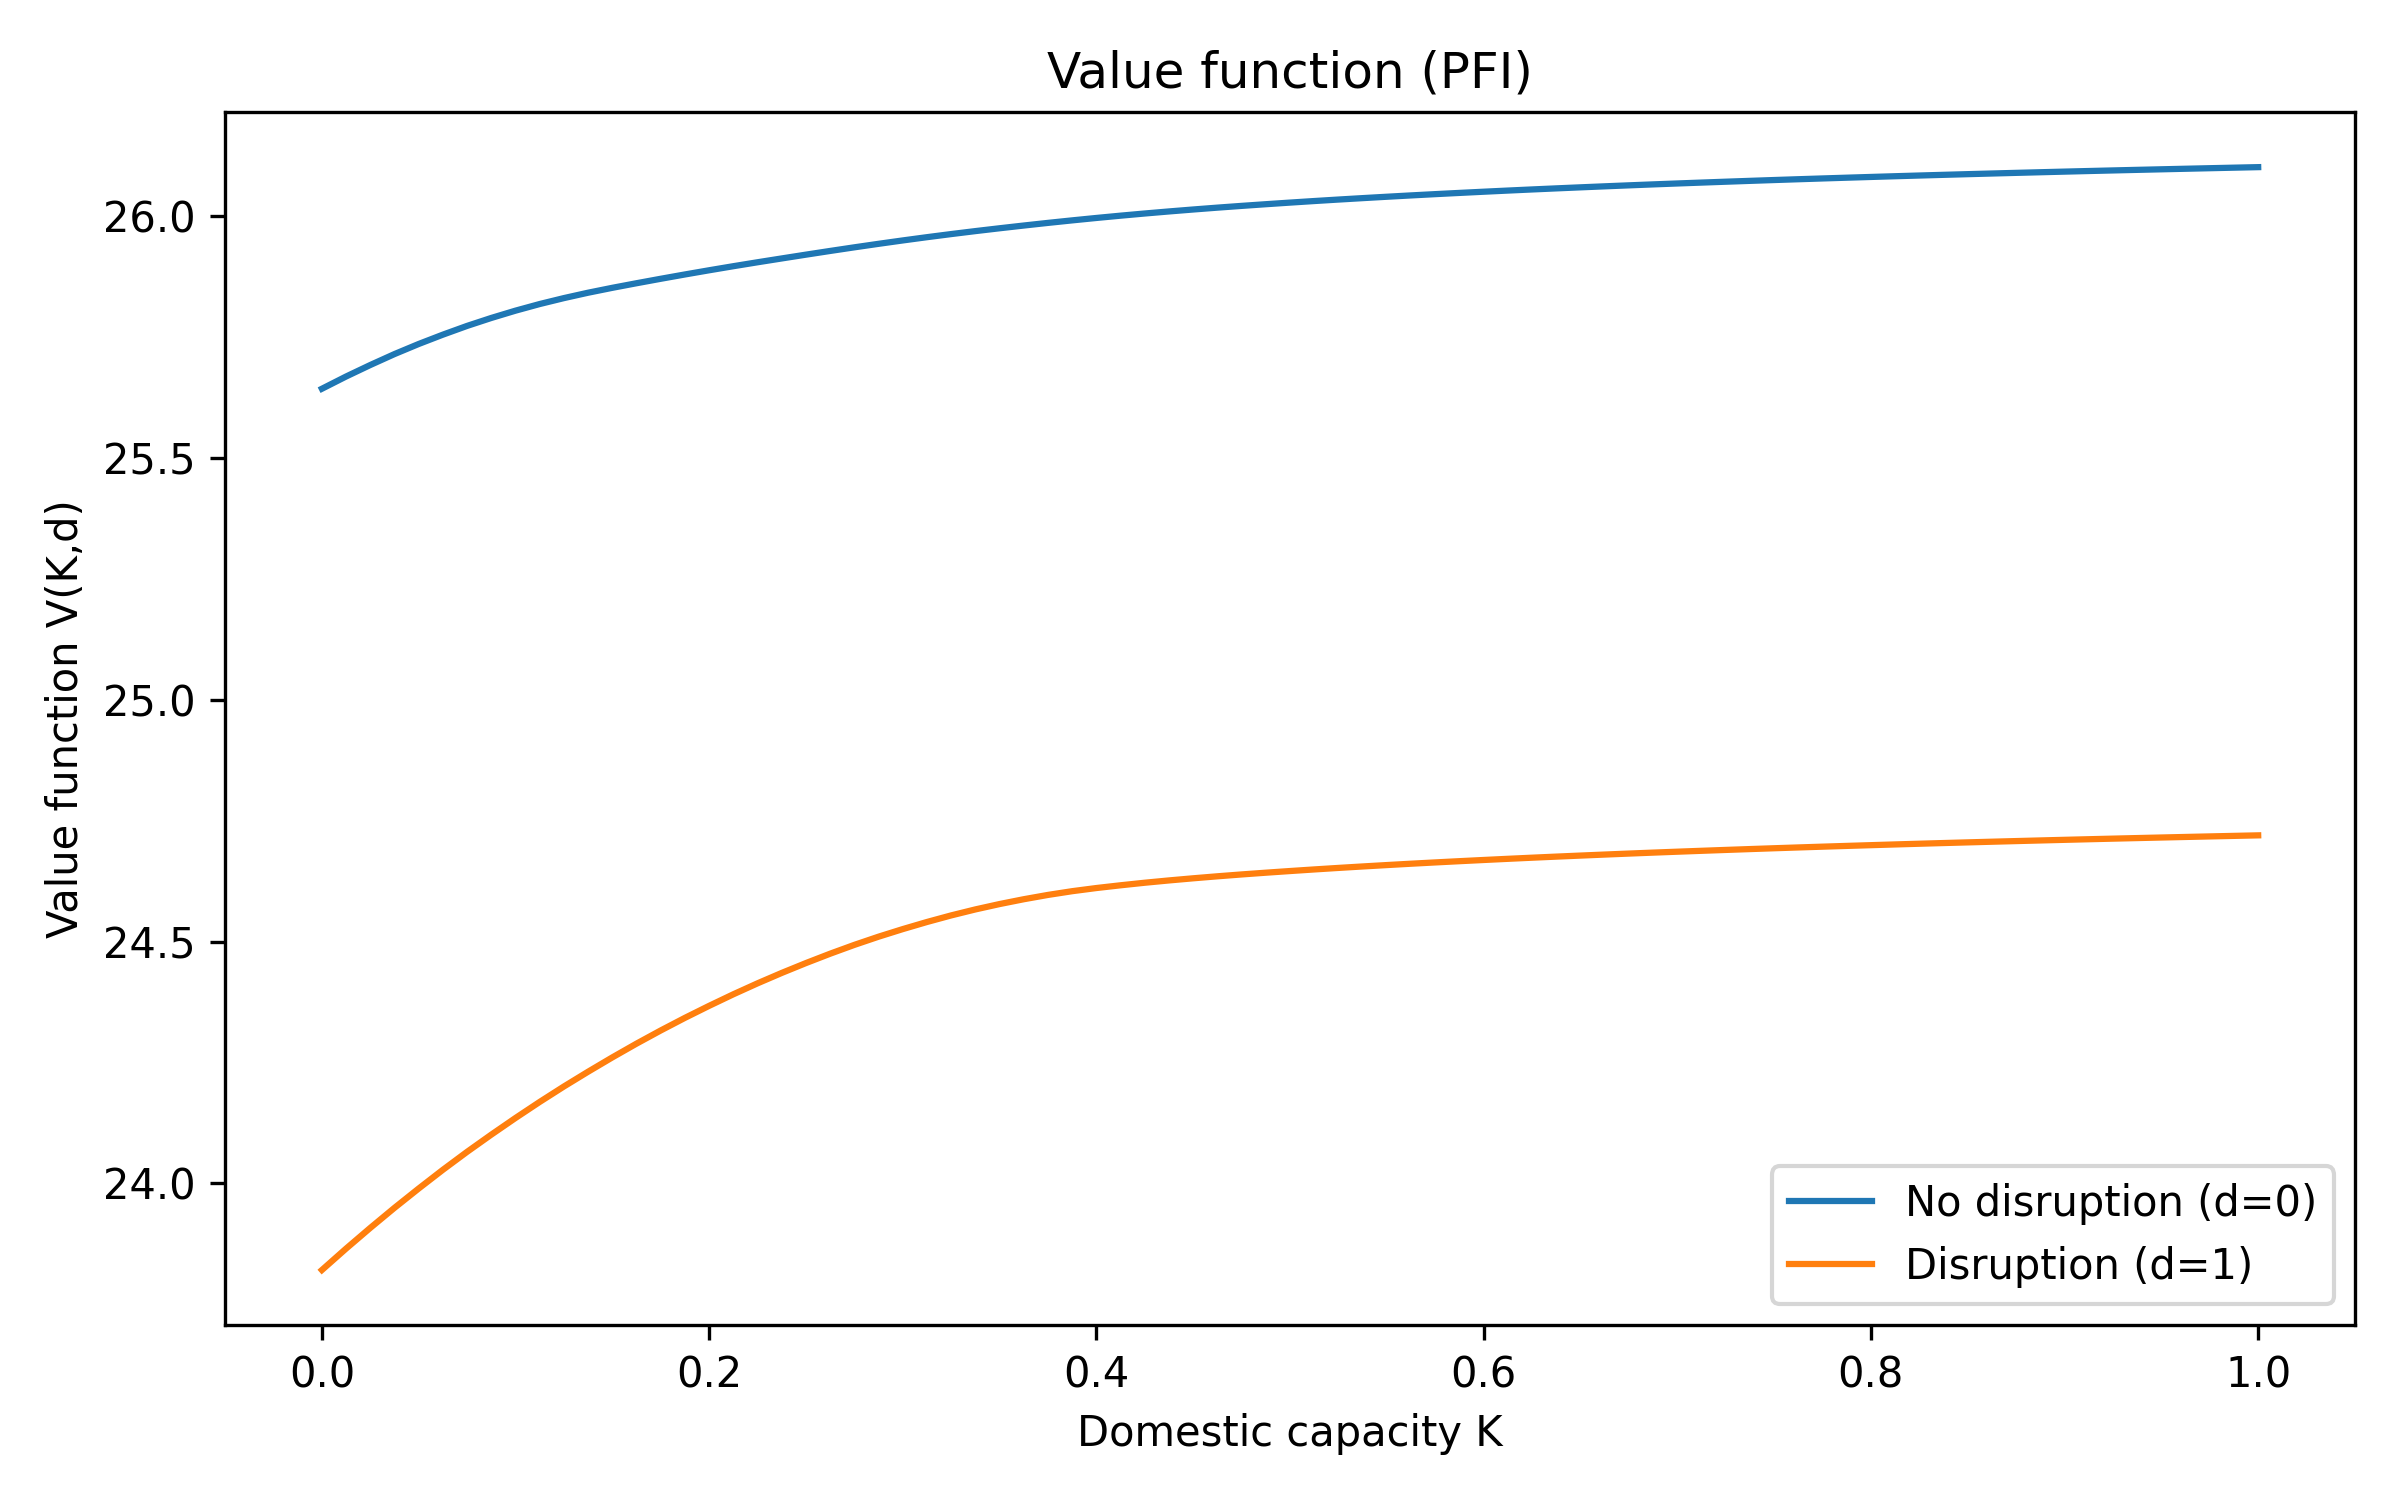
\includegraphics[width=\textwidth]{value_function_pfi.png}
    \end{minipage}
    \caption{Value function comparison: VFI (left) and PFI (right).}
\end{figure}

The value is lower in the disruption state ($d=1$) for all $K$, and increasing in domestic capacity. VFI and PFI deliver nearly identical value profiles.

\subsection{Domestic Sourcing Policy}

\begin{figure}[H]
    \centering
    \begin{minipage}[t]{0.49\textwidth}
        \centering
        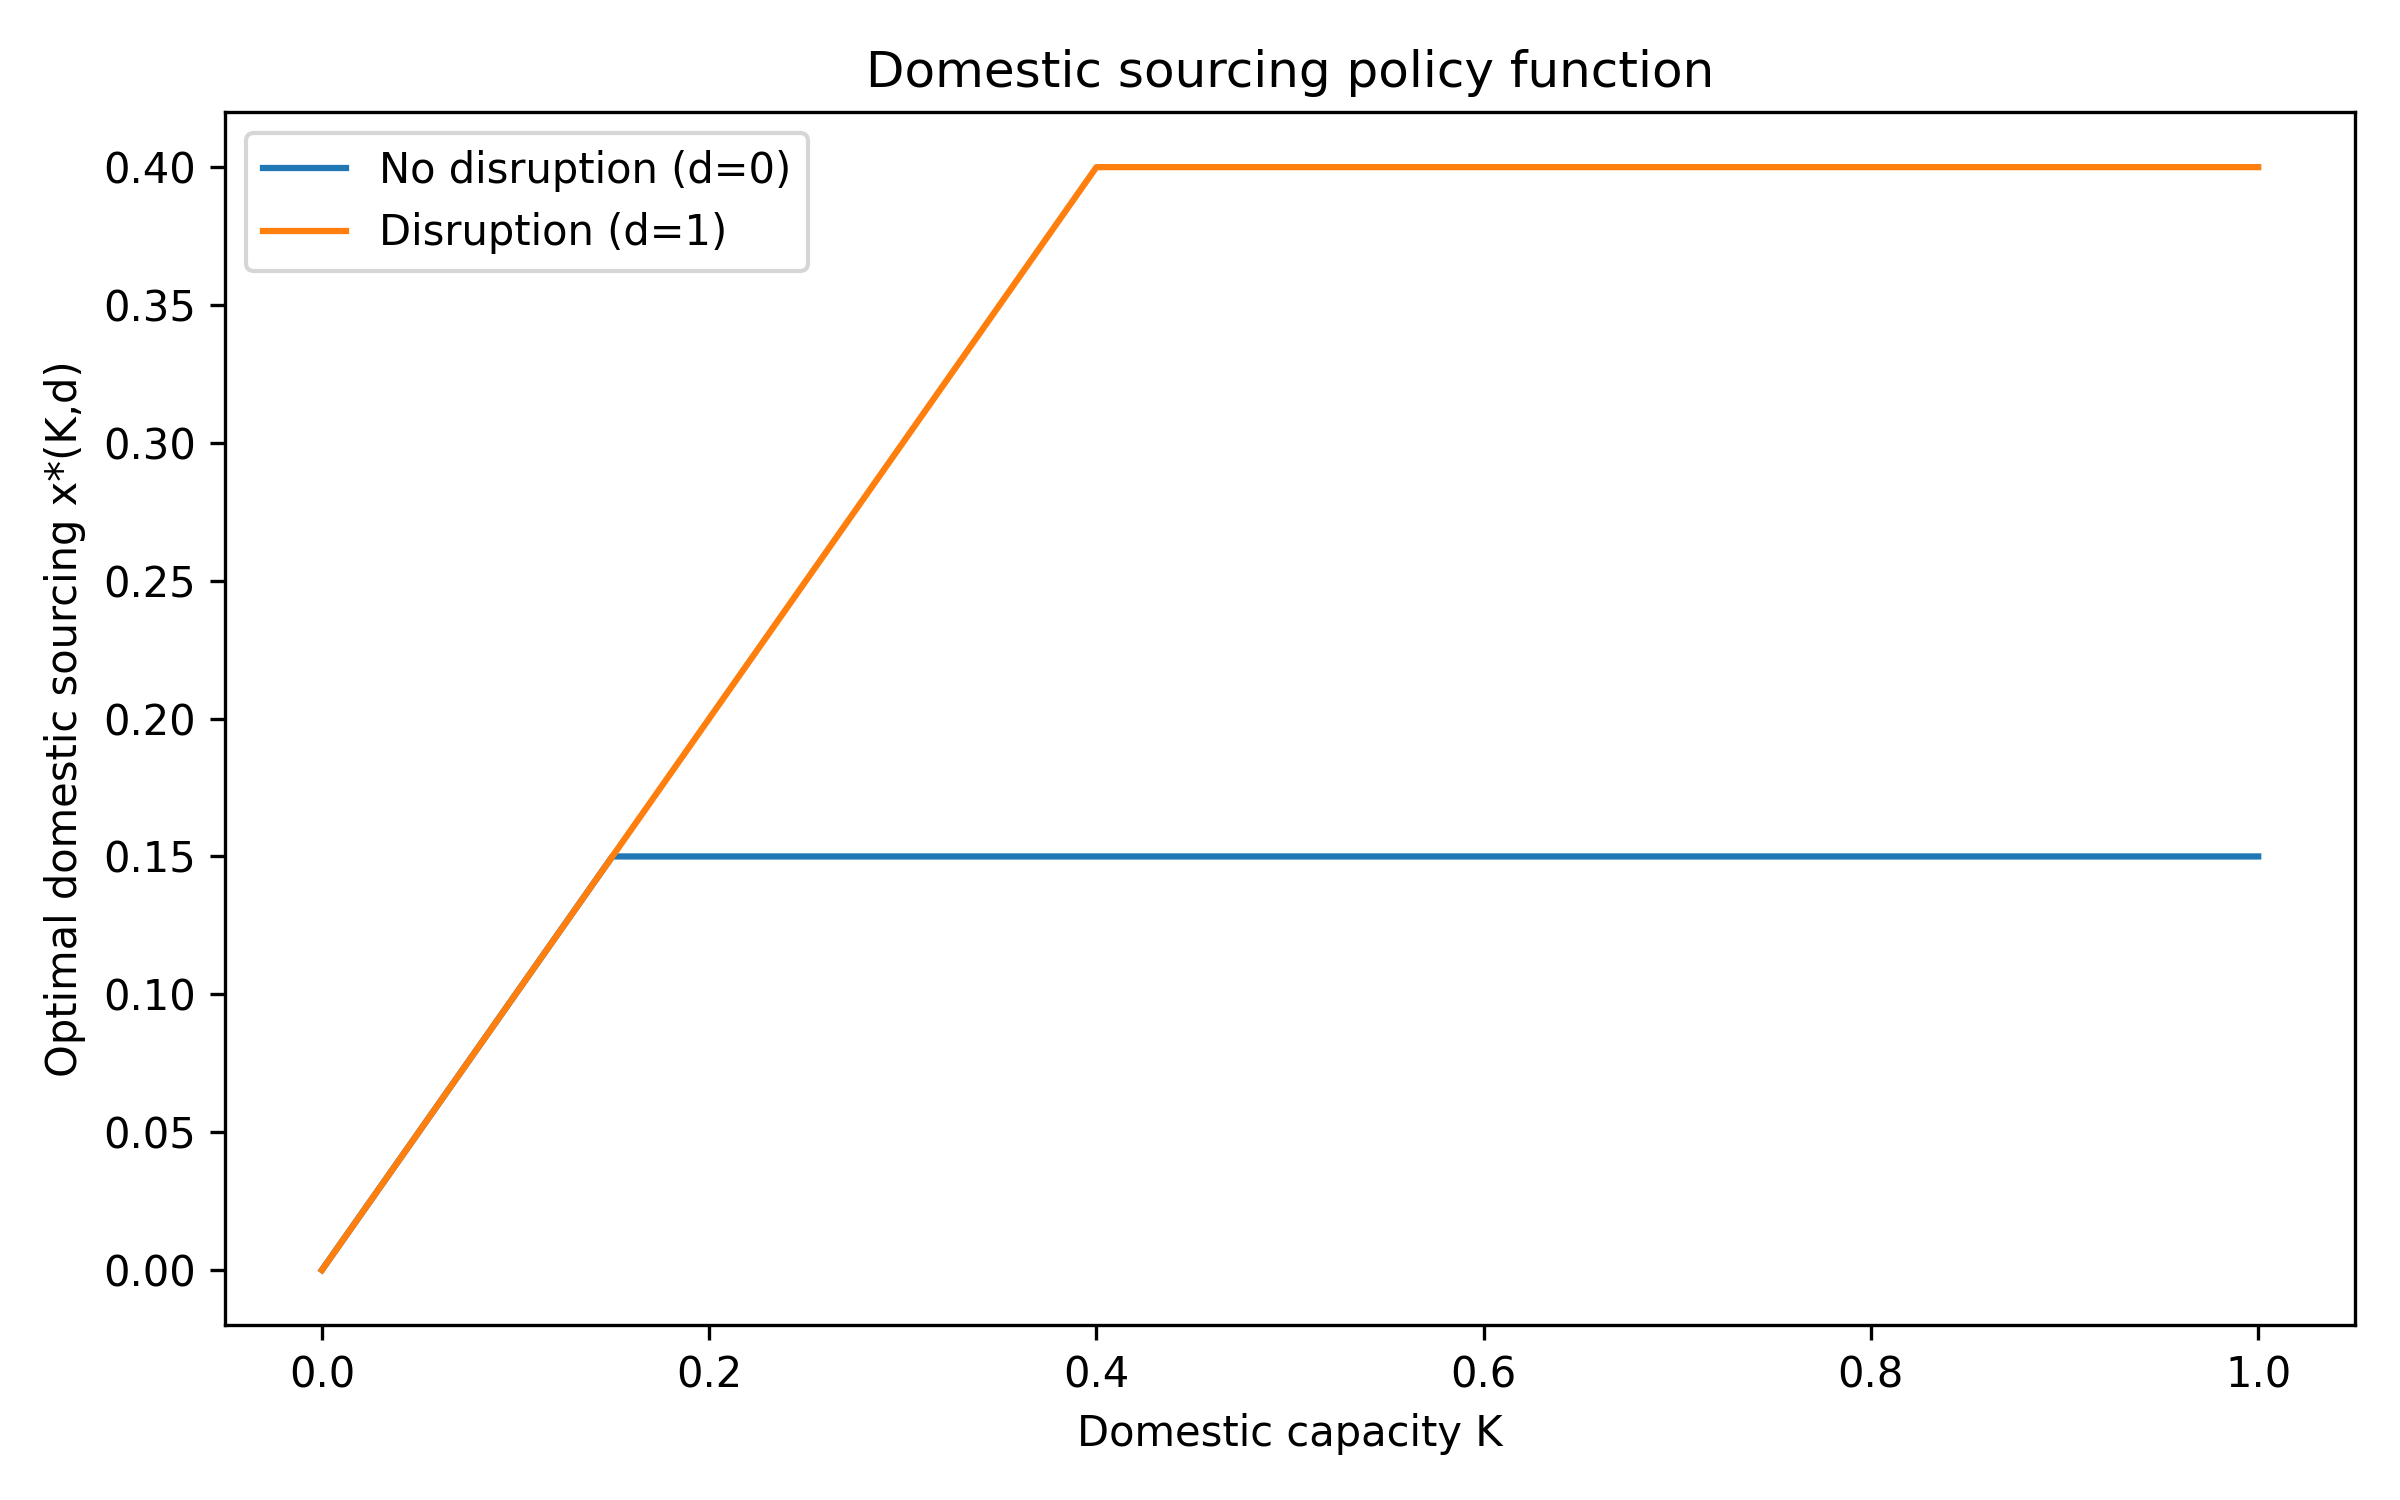
\includegraphics[width=\textwidth]{domestic_sourcing_policy.png}
    \end{minipage}
    \hfill
    \begin{minipage}[t]{0.49\textwidth}
        \centering
        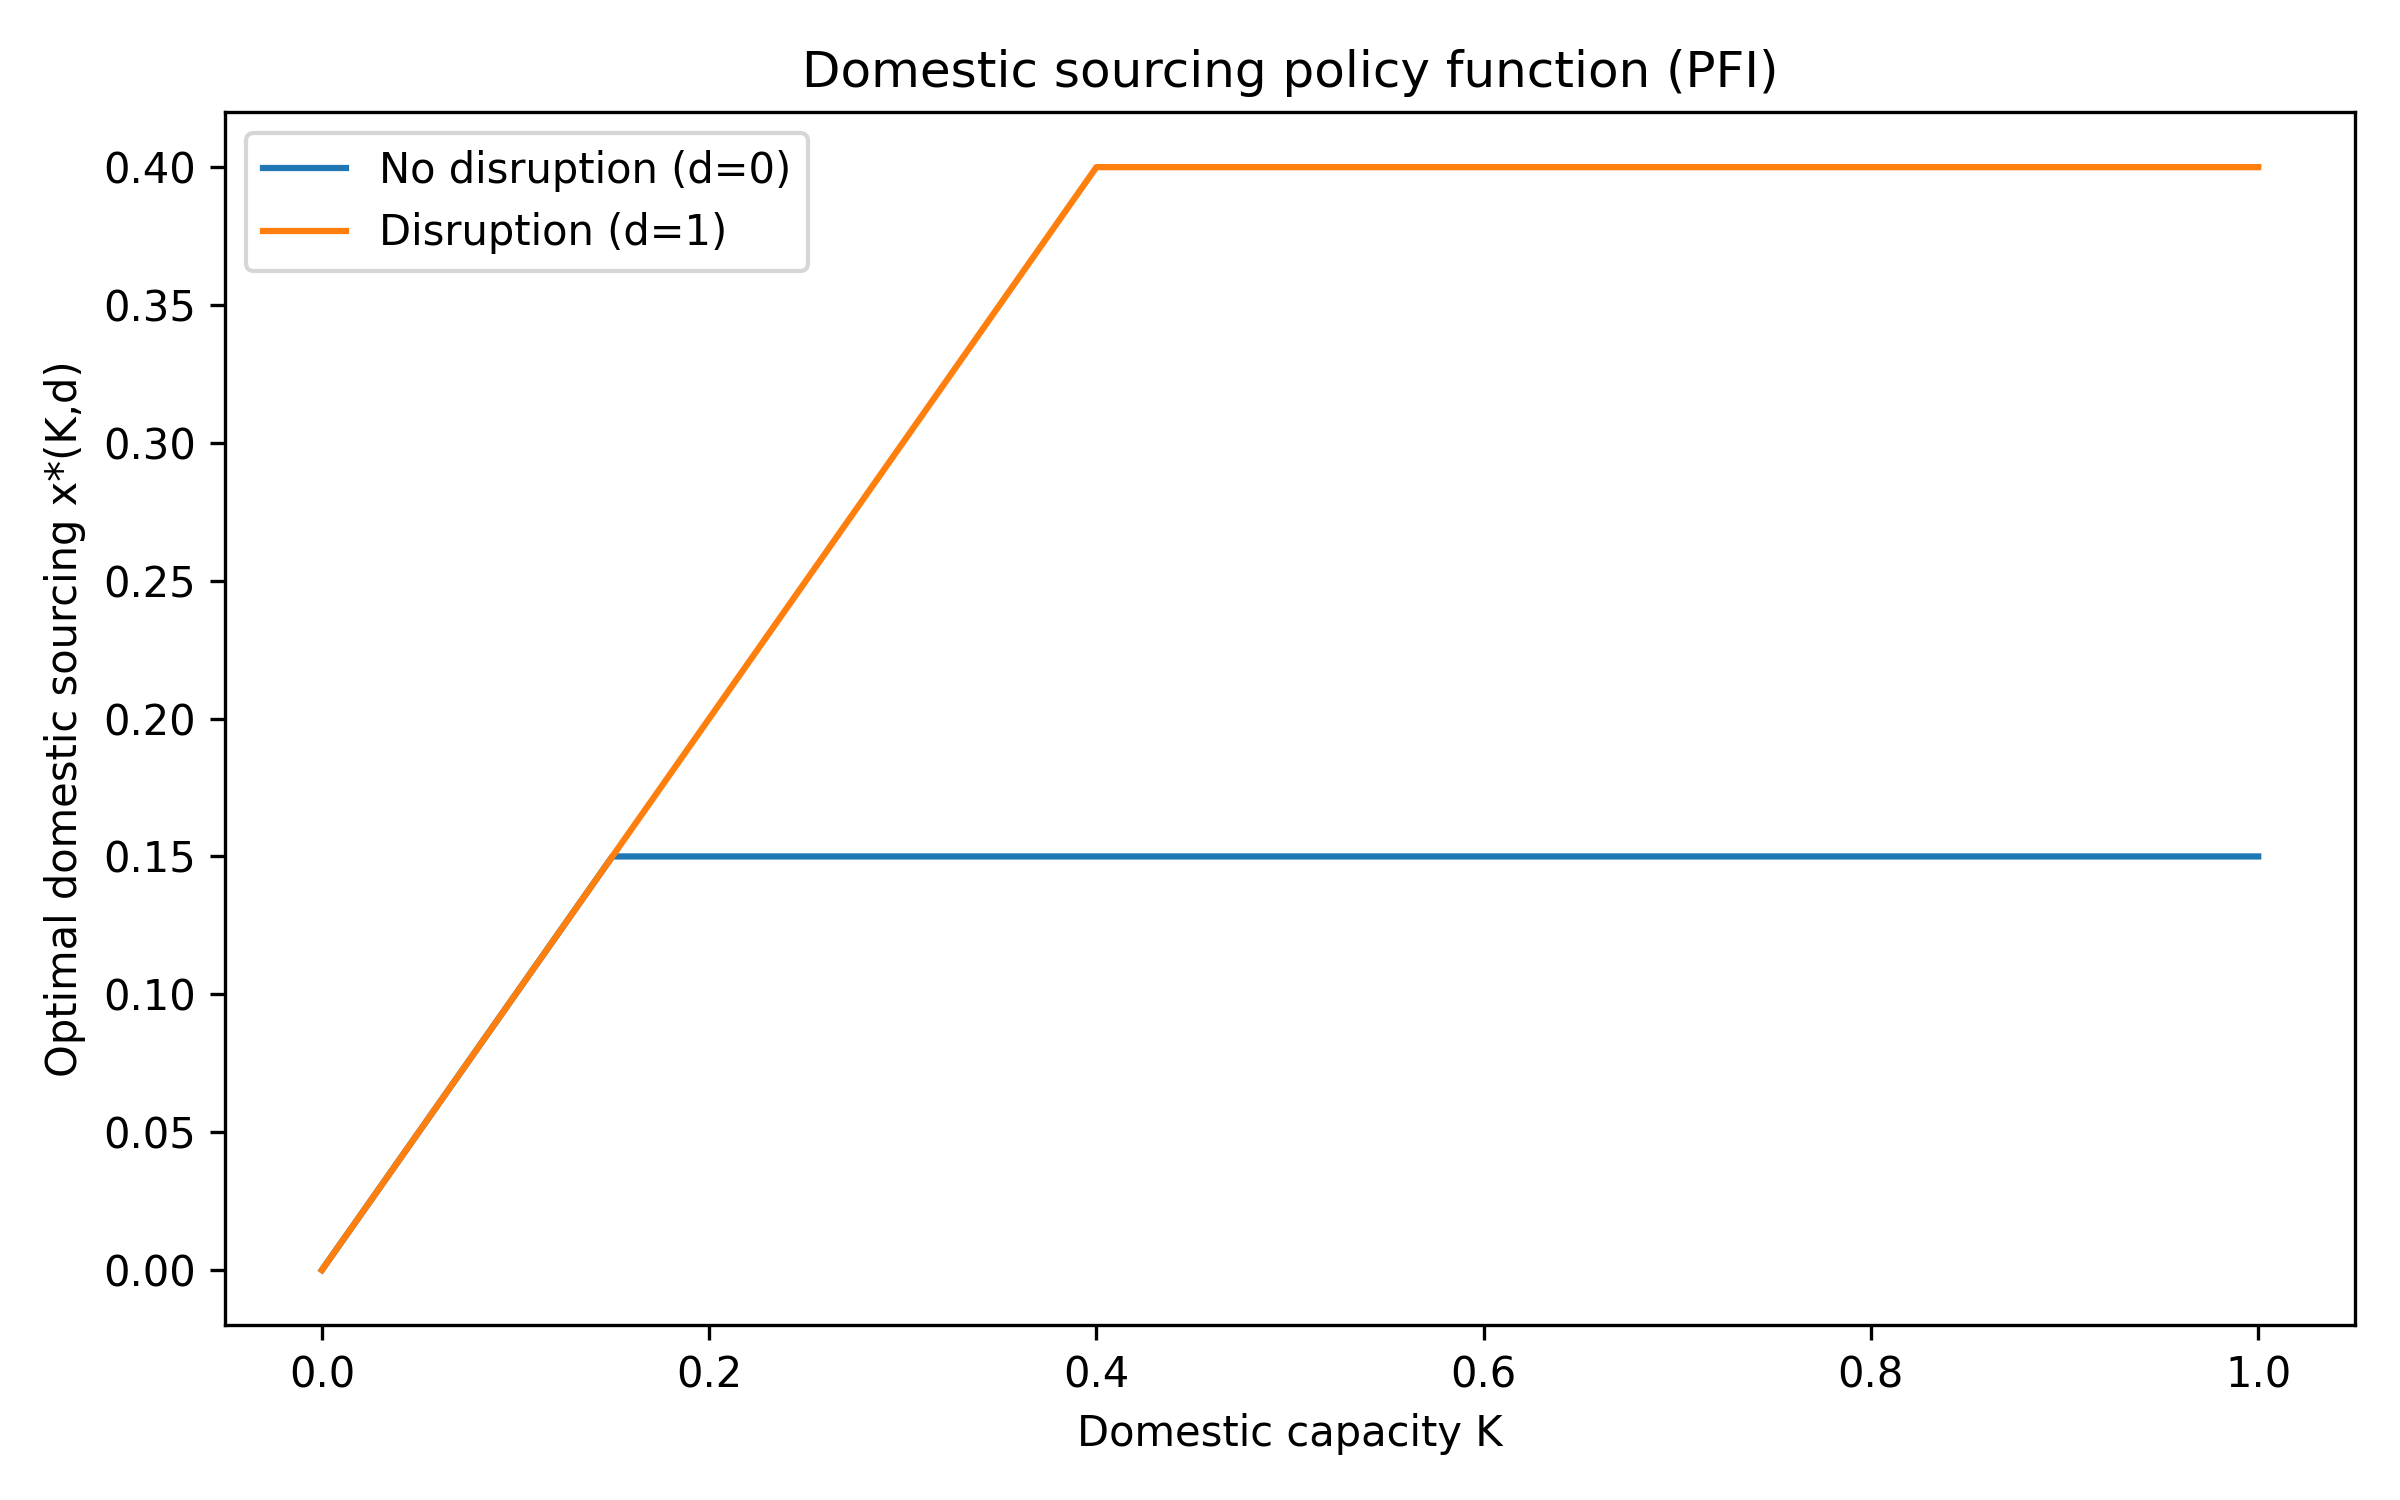
\includegraphics[width=\textwidth]{domestic_sourcing_policy_pfi.png}
    \end{minipage}
    \caption{Domestic sourcing policy comparison: VFI (left) and PFI (right).}
\end{figure}

The policy follows the analytical rule $x^*(K,d)=\min\{K,p_f(d)/c_d\}$. Under disruption, desired domestic sourcing is higher and reaches its cap later as $K$ rises.

\subsection{Subsidy Policy}

\begin{figure}[H]
    \centering
    \begin{minipage}[t]{0.49\textwidth}
        \centering
        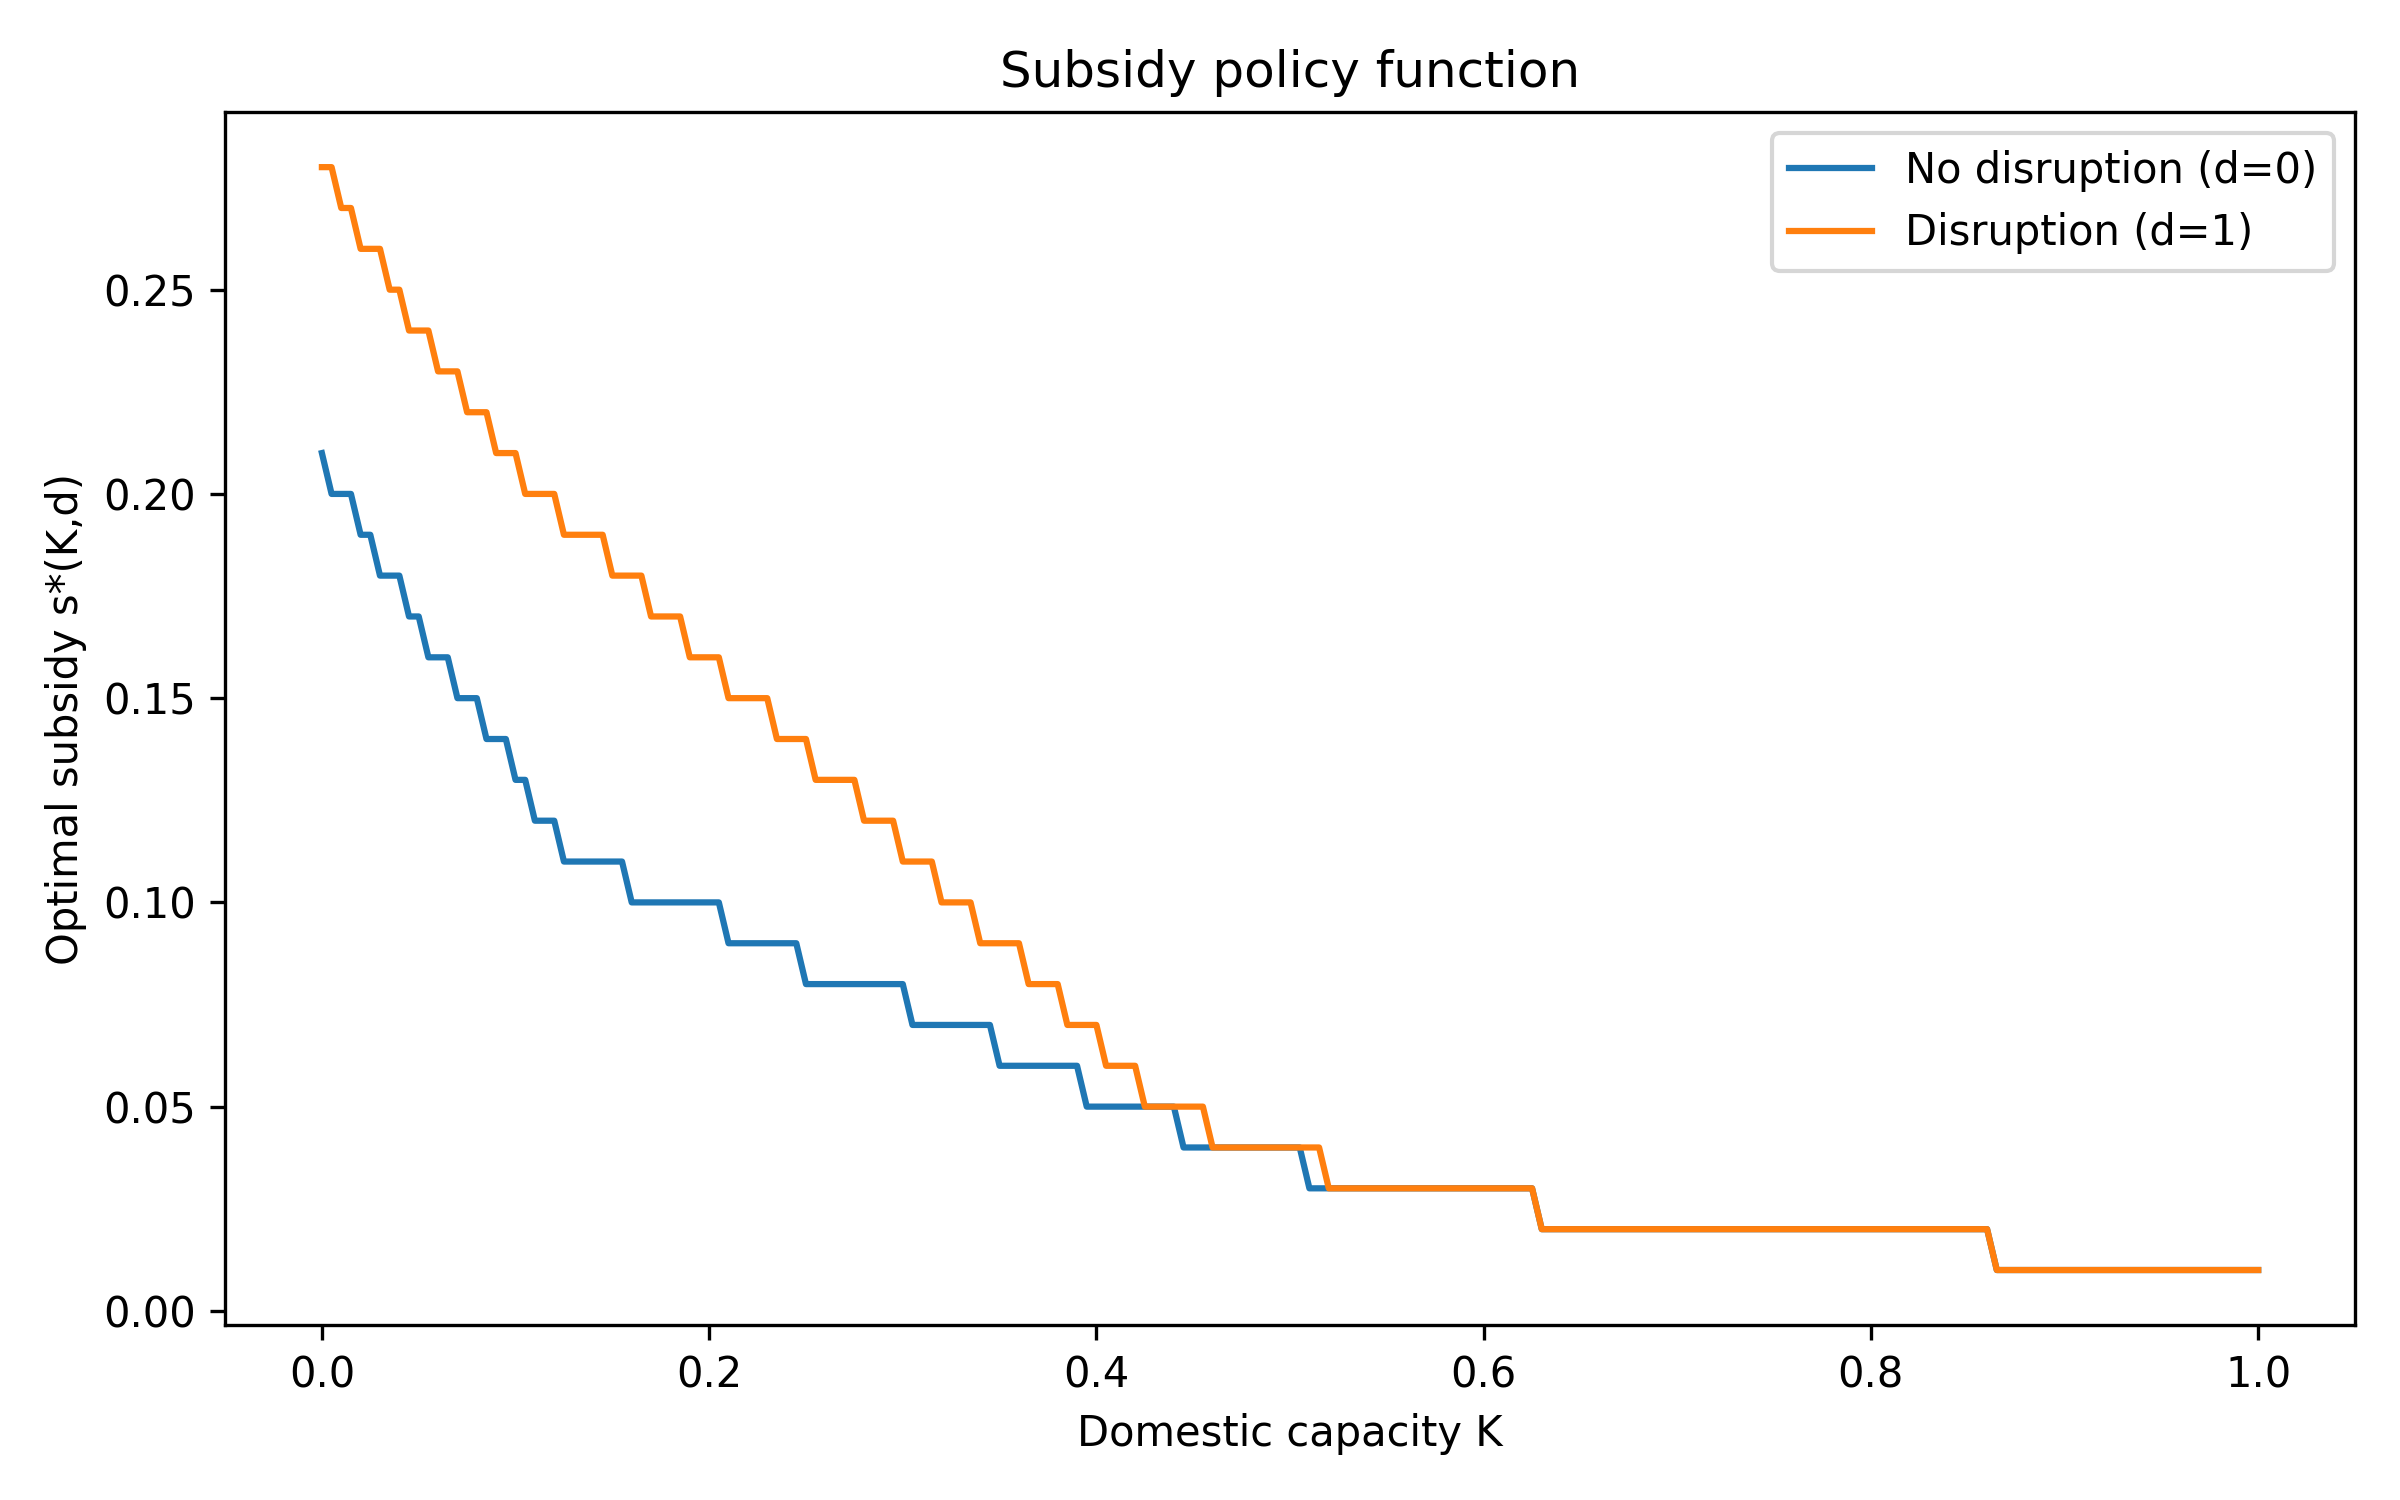
\includegraphics[width=\textwidth]{subsidy_policy.png}
    \end{minipage}
    \hfill
    \begin{minipage}[t]{0.49\textwidth}
        \centering
        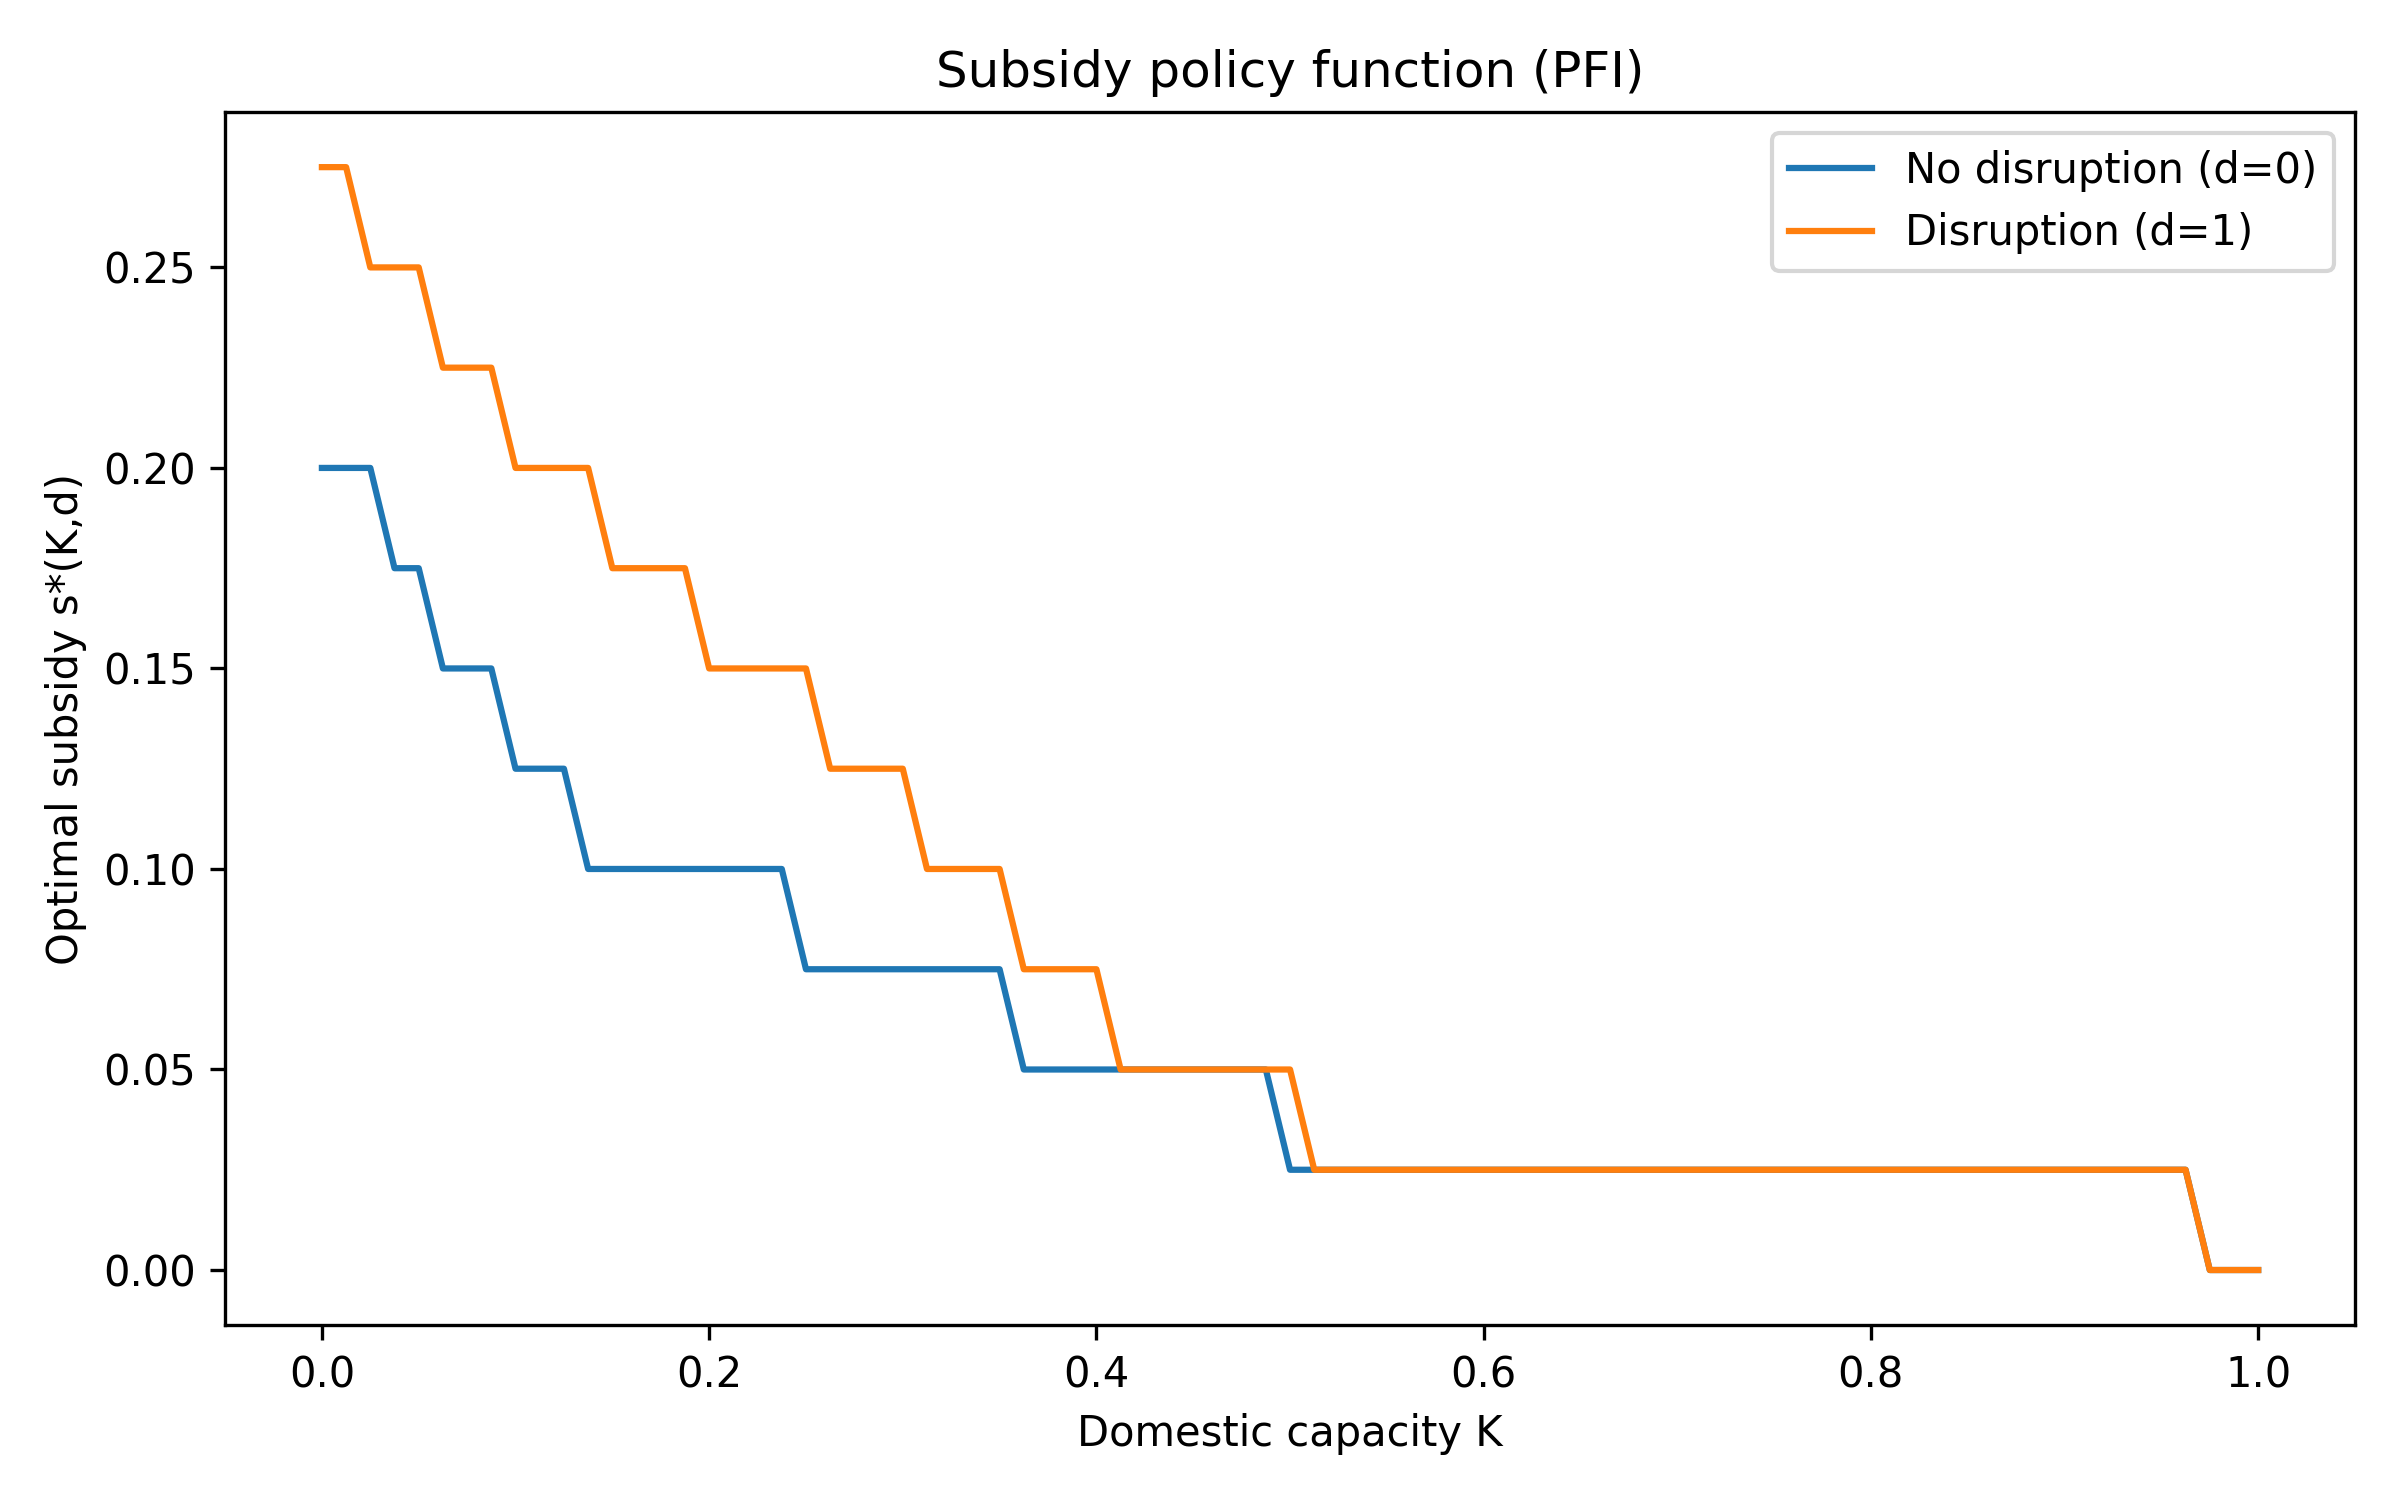
\includegraphics[width=\textwidth]{subsidy_policy_pfi.png}
    \end{minipage}
    \caption{Subsidy policy comparison: VFI (left) and PFI (right).}
\end{figure}

Optimal subsidy effort is decreasing in existing domestic capacity, reflecting diminishing marginal resilience benefits from additional support as the system becomes less constrained.

\subsection{Next-Period Capacity Policy}

\begin{figure}[H]
    \centering
    \begin{minipage}[t]{0.49\textwidth}
        \centering
        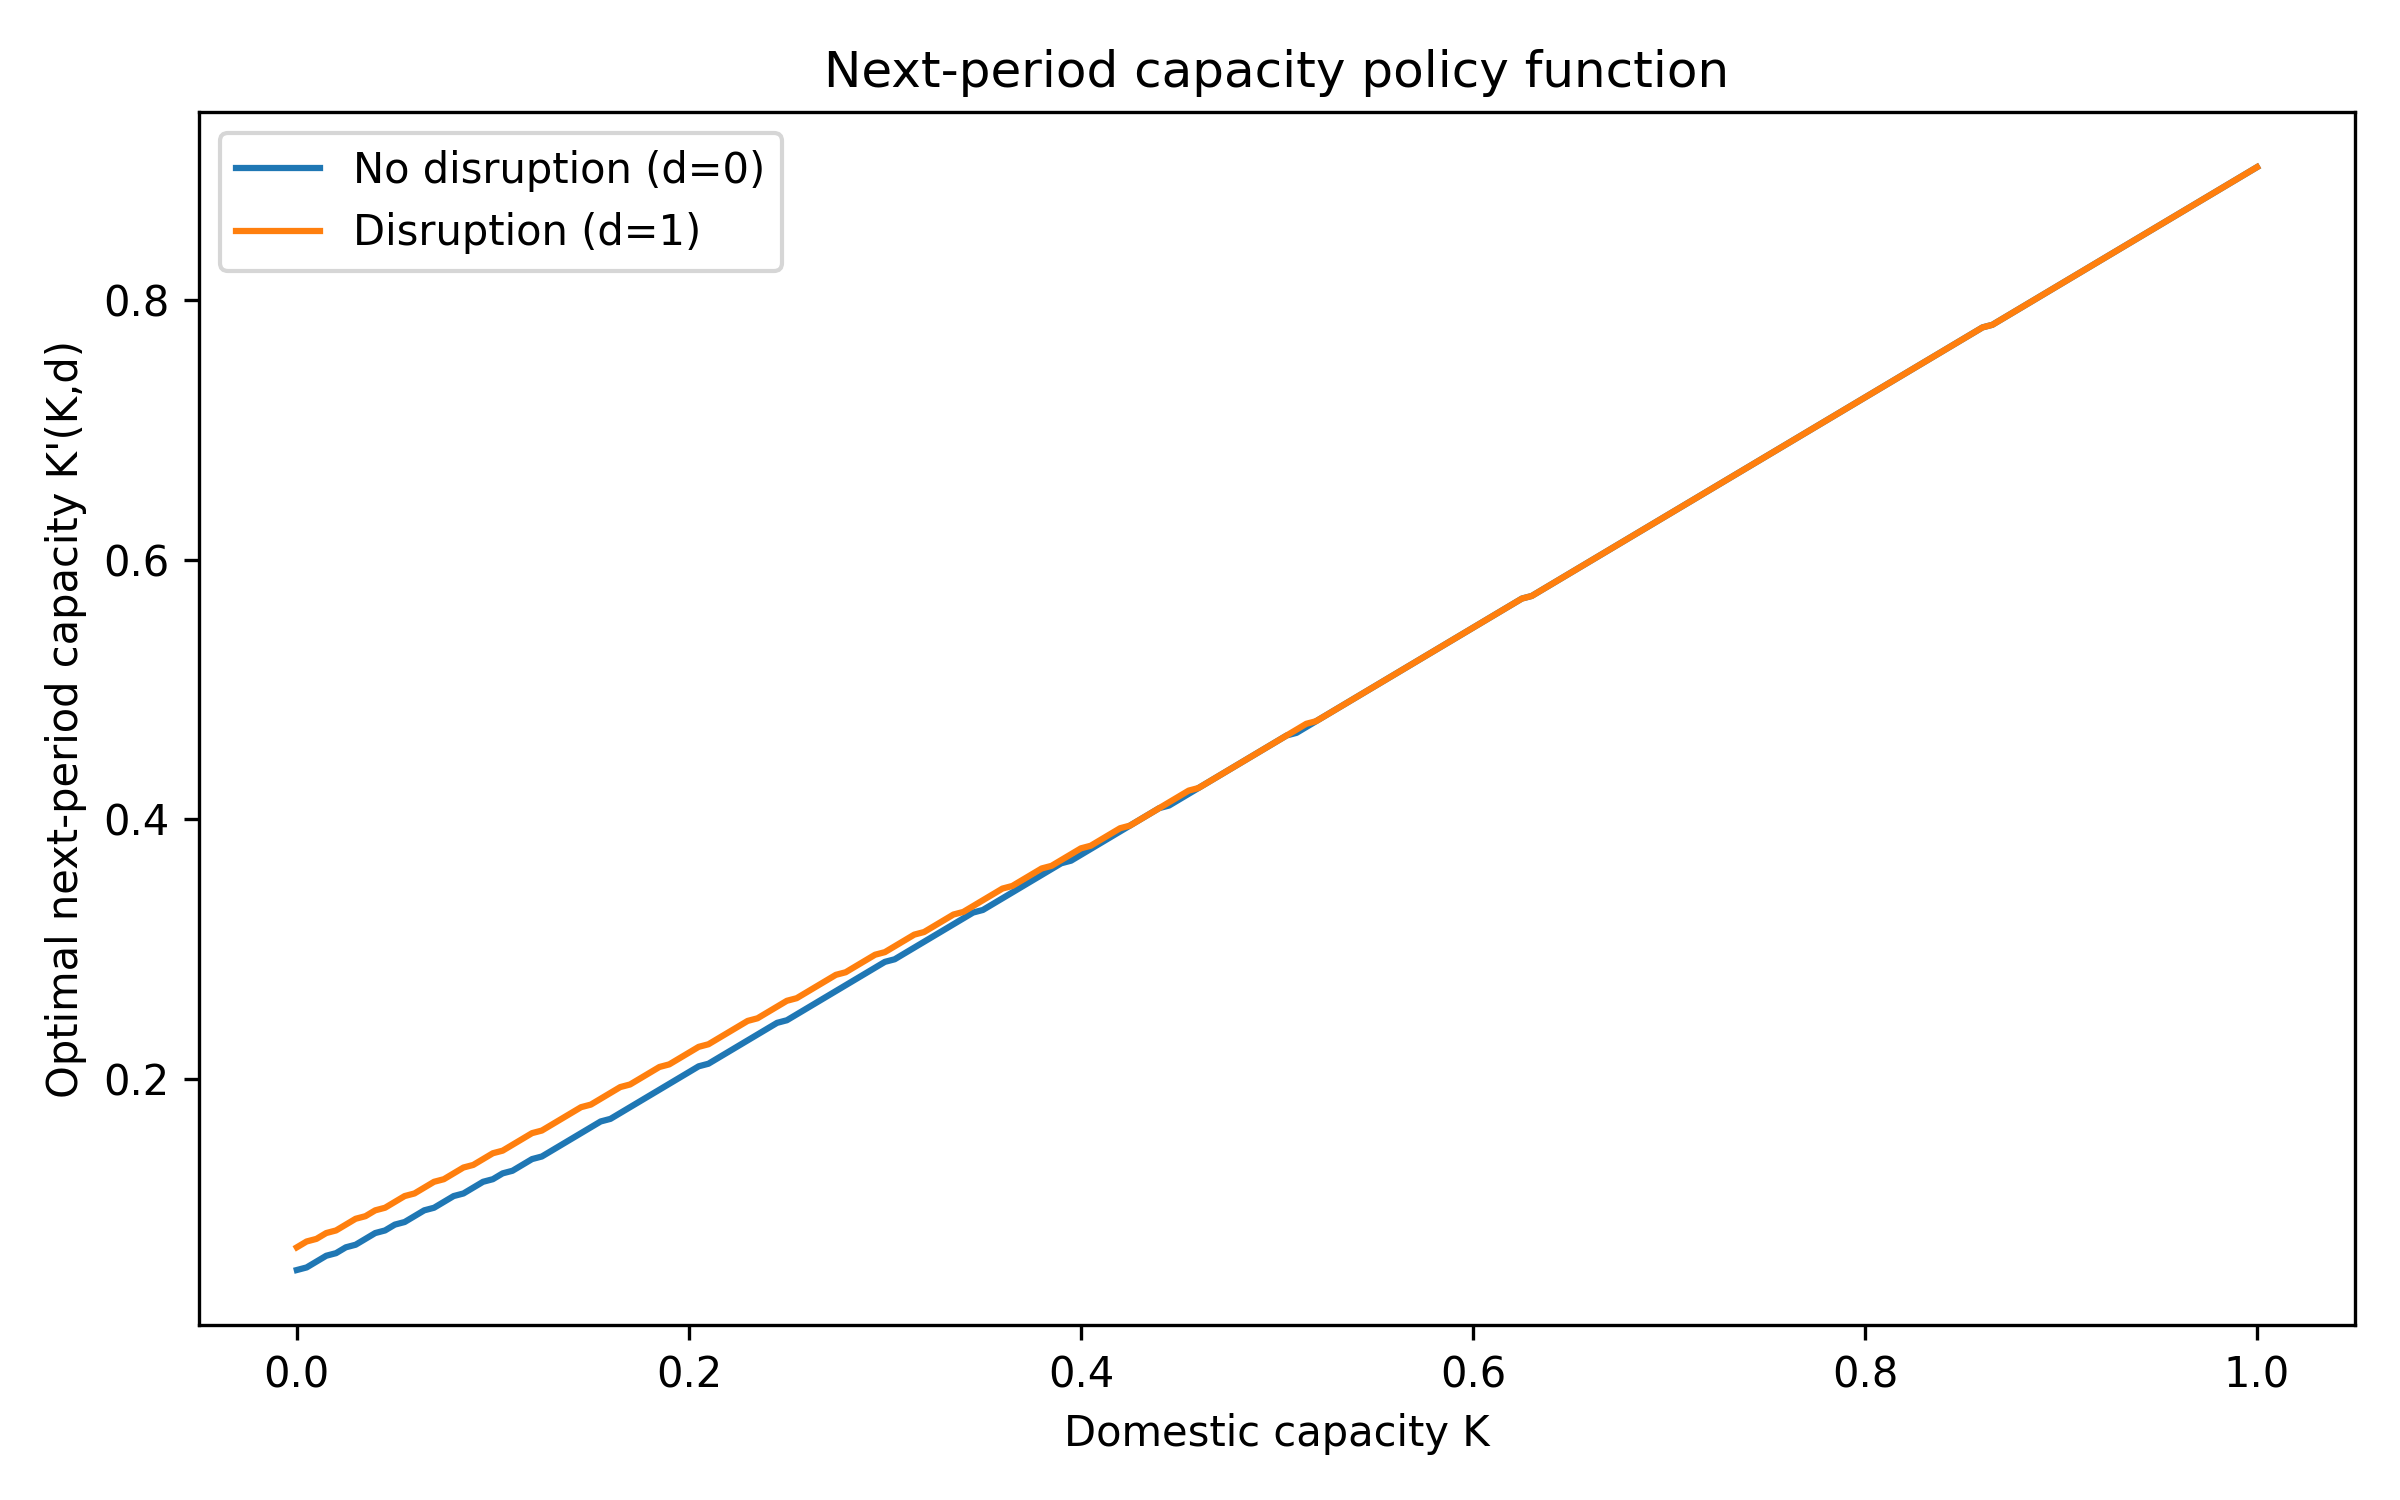
\includegraphics[width=\textwidth]{next_period_capacity_policy.png}
    \end{minipage}
    \hfill
    \begin{minipage}[t]{0.49\textwidth}
        \centering
        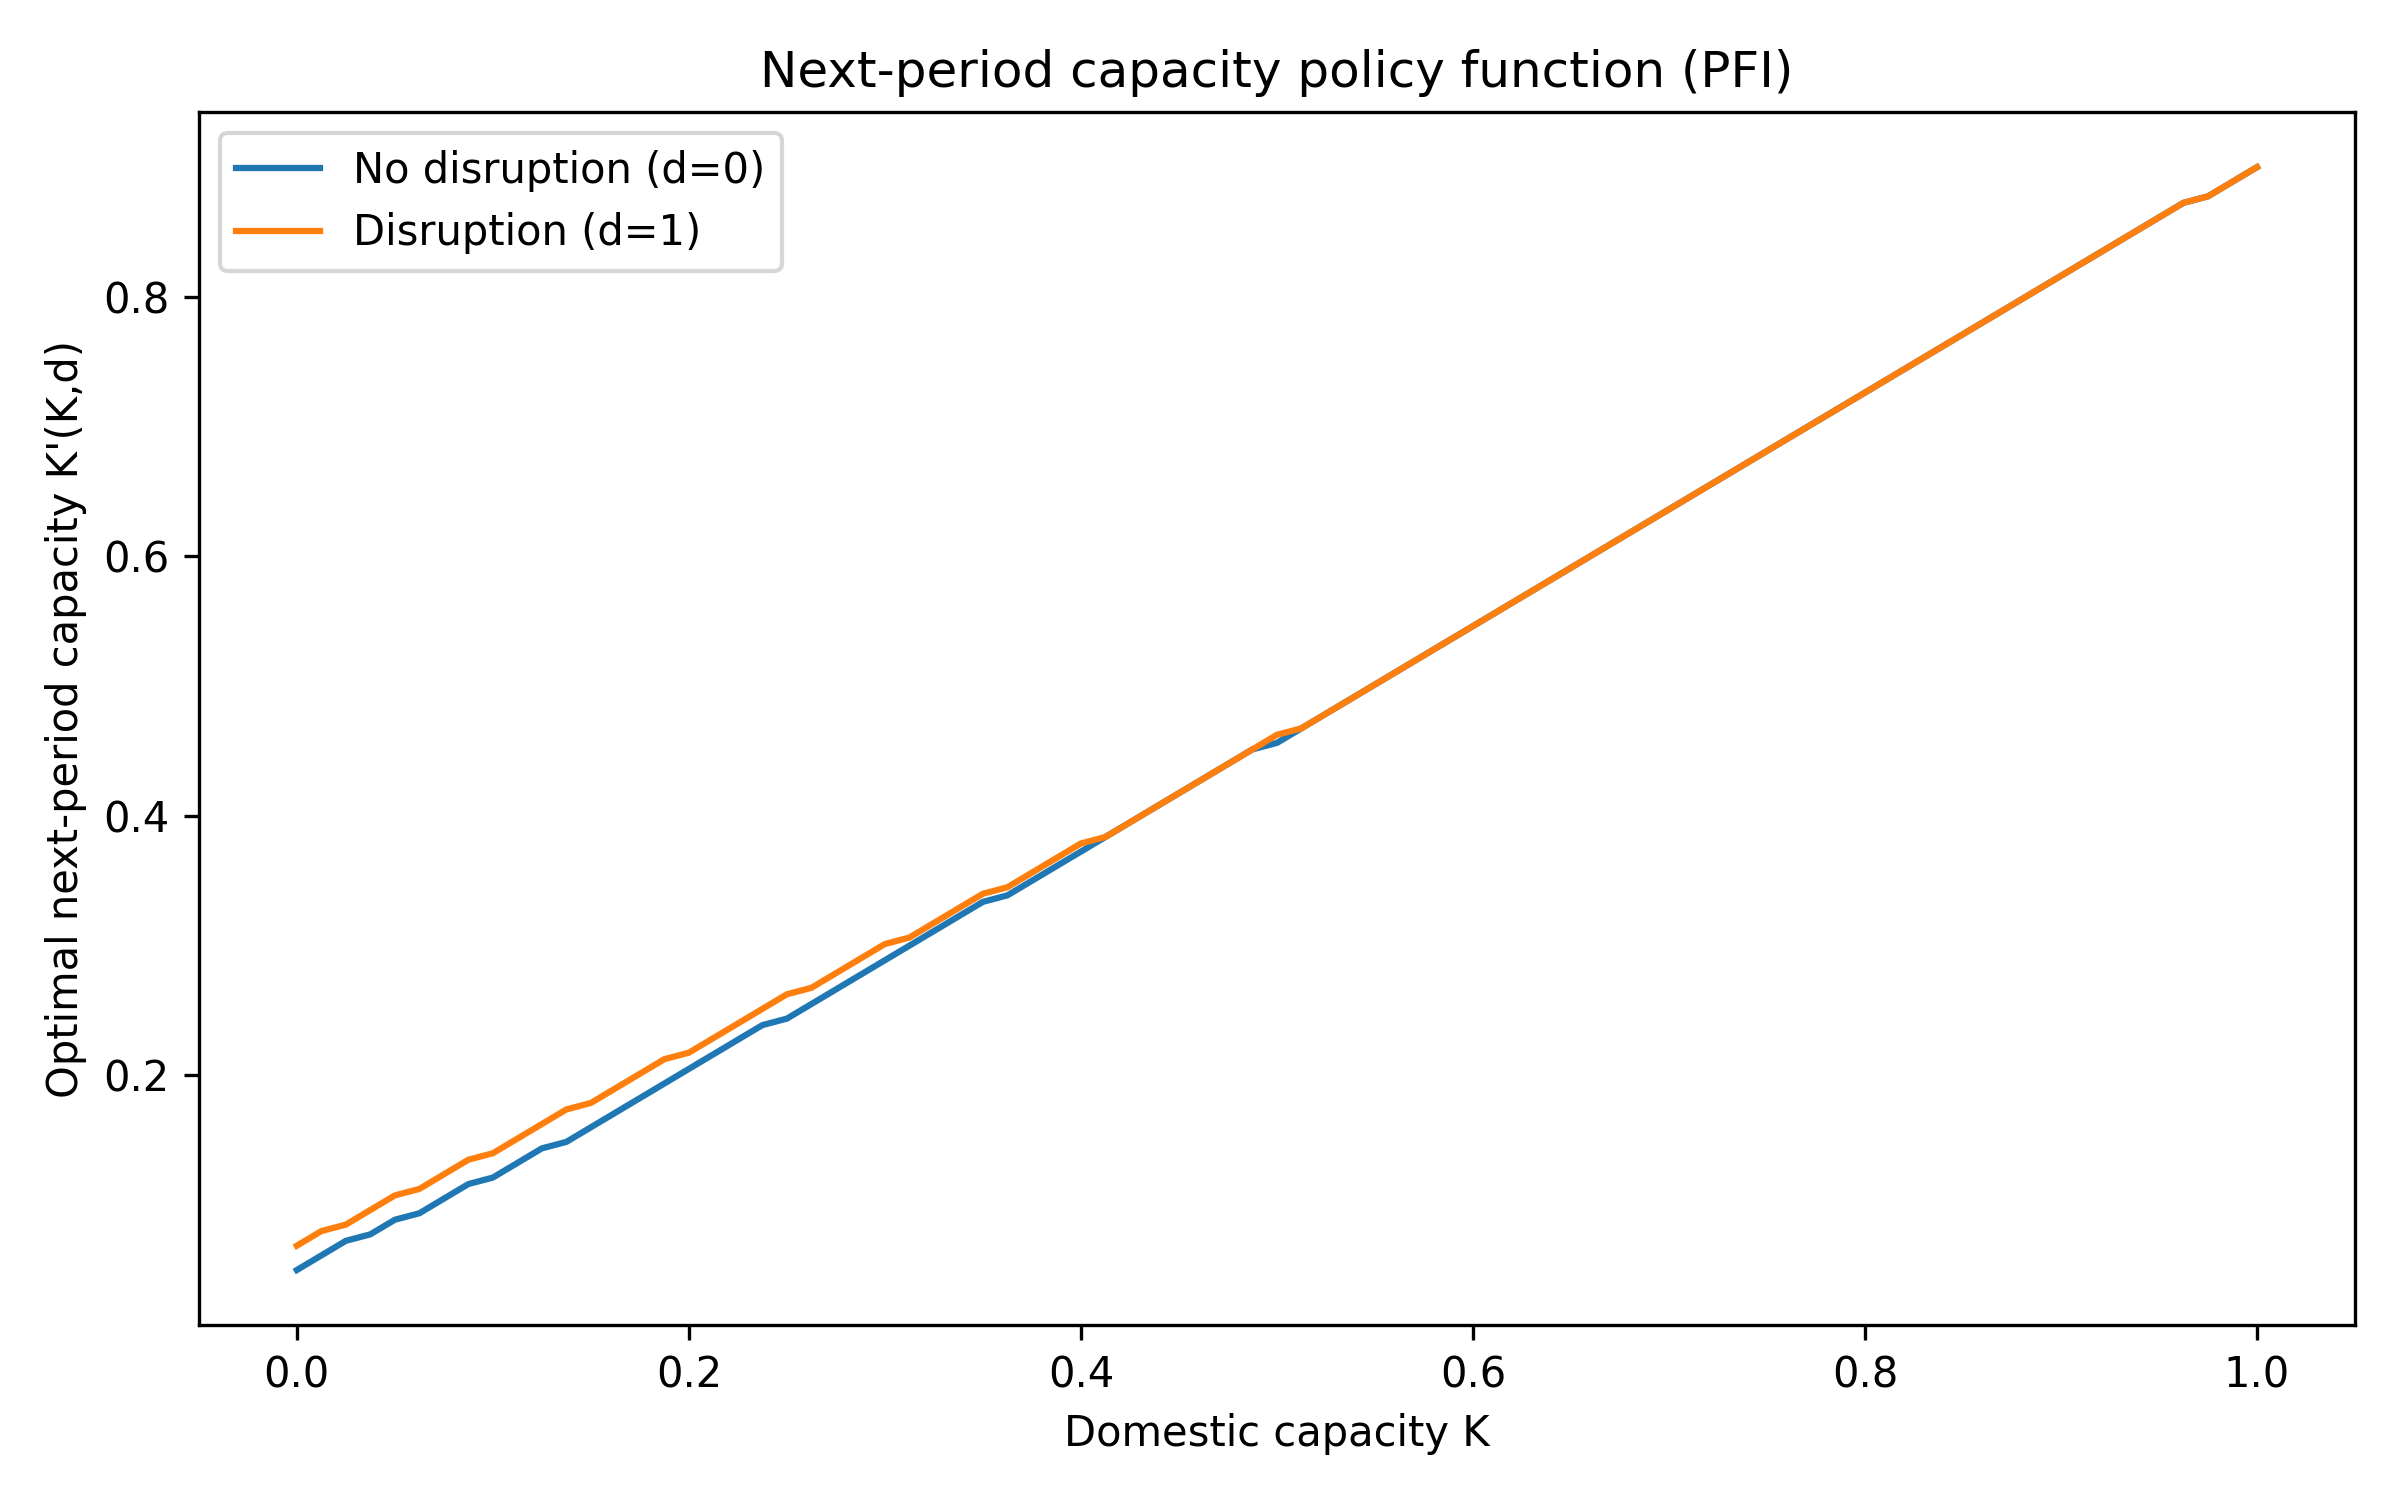
\includegraphics[width=\textwidth]{next_period_capacity_policy_pfi.png}
    \end{minipage}
    \caption{Next-period capacity policy comparison: VFI (left) and PFI (right).}
\end{figure}

The induced law of motion $K'(K,d)$ is increasing in $K$ and very similar across the two numerical methods, with slightly higher accumulation incentives under disruption at low-to-middle capacity levels.

\section{Conclusion}

This model provides a tractable dynamic framework for studying industrial policy under supply-chain risk. The key economic mechanism is simple: foreign sourcing is attractive in normal times, but domestic capacity provides insurance in disruption states. Since capacity is a stock that accumulates gradually, policy has an inherently dynamic character. The Bellman equation, policy rules, and first-order conditions characterize how a planner trades off current fiscal costs against future resilience.

The model is deliberately parsimonious. Relative to the recent literature, it abstracts from multi-tier networks, endogenous supplier-link formation, and decentralized market structure. But this parsimony makes it suitable for dynamic programming and numerical solution in the next problem set.

\begin{thebibliography}{99}

\bibitem[Capponi, Du, and Stiglitz(2024)]{CDS2024}
Capponi, Agostino, Chuan Du, and Joseph E. Stiglitz.
\newblock 2024.
\newblock ``Are Supply Networks Efficiently Resilient?''
\newblock \emph{NBER Working Paper} No. 32221.

\bibitem[Grossman, Helpman, and Lhuillier(2023)]{GHL2023}
Grossman, Gene M., Elhanan Helpman, and Hugo Lhuillier.
\newblock 2023.
\newblock ``Supply Chain Resilience: Should Policy Promote International Diversification or Reshoring?''
\newblock \emph{Journal of Political Economy} 131(12): 3462--3496.

\bibitem[Grossman, Helpman, and Sabal(2024)]{GHS2024}
Grossman, Gene M., Elhanan Helpman, and Alejandro Sabal.
\newblock 2024.
\newblock ``Optimal Resilience in Multi-Tier Supply Chains.''
\newblock \emph{Quarterly Journal of Economics} 139(4): 2377--2425.

\end{thebibliography}

\end{document}